\chapter{Thesis boundaries}
\label{chapter 3}
\ifpdf
    \graphicspath{{Chapter3/Figs/}{Chapter3/Figs/PDF/}{Chapter3/Figs/}}
\else
    \graphicspath{{Chapter3/Figs/Vector/}{Chapter3/Figs/}}
\fi
Production systems can take a wide variety of forms, depending on the specific type of application. Generally, the proper way to explore how to address a problem using a new approach is to start from relatively simple contexts, delineating the dissertation boundaries. \\
This chapter defines the thesis areas of interest, concerning the type of production systems, the sensor positions and the types of variations assumed to occur during the process. Before the boundary definitions, a description of the event logs is provided, in order to illustrate their structure and to show what information they can carry. 
\section{Event logs}
\label{Event logs}
An event log is a data table where each row records a single event occurred during a specific process. Events are sequentially registered such that, at least, each one is associated to the case (i.e., a process instance, a job) object of the event, and with the activity (i.e., a well-defined step in the process, e.g. entering in a buffer, starting the production) performed on the case \cite{BoseR.P.JagadeeshChandra2013Wipm}. \\ 
Thus, if the event order is preserved, a minimal event log (called simple event log) is composed of only two fields, containing the following information 
\begin{itemize}
\item \textbf{ID of the case}: the code that uniquely identifies a certain case flowing in the process. 
\item \textbf{ID of the activity}: the code that uniquely identifies a certain activity performed on a case
\end{itemize}
With these three information (including the event order) a trace can be extracted for each case, which is the ordered sequence of activities executed on a case. So, a simple event log can be reorganized as a multi-set of traces over a set of activities.\\
However, in general, event logs are composed by more fields containing different case attributes or event attributes, which allow a deeper and more meaningful analysis of the process.
\begin{figure}[H] 
\centering    
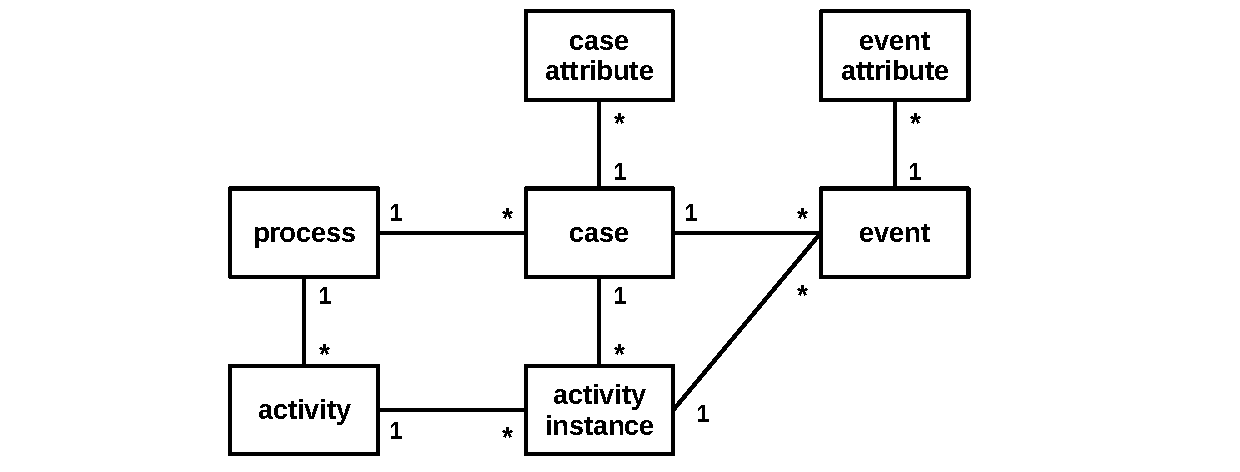
\includegraphics[width=1\textwidth]{Event_log_class_diagram_2}
\caption[Event log class diagram]{Event log class diagram \cite{Aalst16}}
\label{fig:Event log class diagram}
\end{figure}
Figure \ref{fig:Event log class diagram} displays the class diagram of the components of a general event log. The main structure of simple event logs is still present in richer event logs:
\begin{itemize}
\item Each event log refers to only one process
\item Each case belongs to one process but a process may consist of many cases
\item Each event refers to one case but a case may be the subject of many events
\item Each activity may be performed on many cases and each case may be processed by different activities
\end{itemize}
The diagram shows that, in general event logs, in contrast to simple event logs, cases and events may have many attributes. Some examples are
\begin{itemize}
\item \textbf{Timestamp}: an event attribute containing the instants when events verified
\item \textbf{ID of the resource}: an event attribute containing the codes that identify which resources (e.g. an operator that performs different activities, a machine in a multi-machine stage) were utilized to process the job
\item \textbf{Cost}: an event attribute containing the costs related to events
\item \textbf{Case type}: a case attribute registering the category to which the case belongs, useful in a multi-product system context
\end{itemize}
The presence of attributes allows to apply Model Enhancement algorithms, which aim to create models that look at a process from different perspectives. For example, if the resource ID\footnote{In this case, intended as the operator IDs} is available, it is possible to generate graphs of the social network, that show the employee relationships, the work sequence and the connection frequency. 
\subsection{Event logs in real applications: event streams}
In manufacturing, event logs are the output produced by sensors positioned along the production line. The sensor locations are determined a priori, and the sensors should guarantee a good level of reliability to minimize errors in the event log.\\
As explained in section \ref{Auto-update of process models using Process Mining}, in real applications, often, events are collected one at a time, generating event streams, however this thesis only considers event logs consisting of complete datasets, while the event stream situation is not explicitly taken into account. This simplification causes a partial, but not total, generality loss with respect to the event flow case. Indeed, this dissertation has the aim to clarify if it is possible to detect and identify some specific types of variation. Concerning the change detection, since this issue is addressed by assessing the event log with an event-by-event (or window-by-window) approach, that is comparing each new event with the previous ones, the dataset completeness is not necessary and the same approach could be also applied in an event stream context without any adaptation. Instead, regarding the change identification, the event log completeness is much more relevant. To understand what kind of variation is occurring, a simple comparison of consecutive events is insufficient, and the complete event log case and the event stream case lead to different approaches. In the first case (if the event log includes an enough long collection of after-change events), the dataset serves as a snap-shot of the process, making easy to recognize steady state periods before and after the variation and allowing to directly compare them to get insight about the process evolution. Instead, the second case, which necessarily works collecting events (or event windows) one at a time, must also deal with the problem of identifying when the process reaches again the steady state after the variation. \\
Therefore, while reasonings about the change detection can also be straight applied to event stream situations, even if the study only considers complete event logs, the change identification presents additional challenges that are not addressed in this thesis. 
\section{Considered systems}
\label{Considered systems}
\subsection{Simple serial lines (SSLs)}
In this thesis the considered systems are limited to Simple Serial Lines (SSLs), also called basic straight lines, with one resource for each of stage. 
\begin{figure}[H] 
\centering    
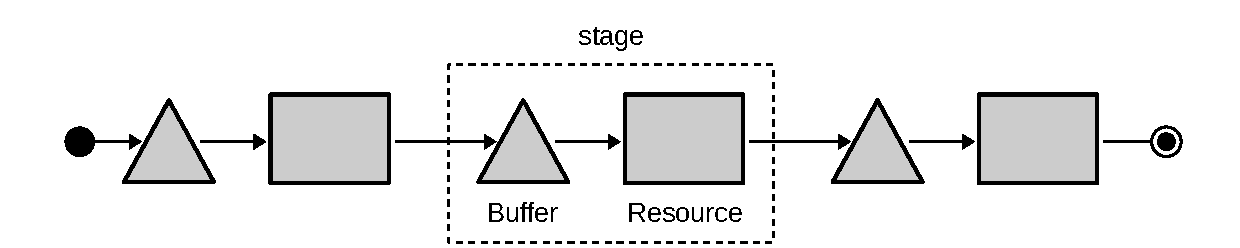
\includegraphics[width=1\textwidth]{SSL_scheme}
\caption[A SSL composed of three stages]{A SSL composed of three stages}
\label{A SSL composed of three stages}
\end{figure}
Figure \ref{A SSL composed of three stages} shows an example of a SSL made of three stages, each one composed of a buffer and a resource. SSLs are described in \cite{Romero-SilvaRodrigo2019Splp}, having the following characteristics.
\begin{itemize}
\item \textbf{Production in discrete parts}\\
Discrete manufacturing involves finished products consisting of distinct items (or batches of items) that can be counted, touched, or seen. Production is guided by a bill of materials (BOM) and follows a route, such as an assembly line. Examples of discrete manufacturing products are automobiles, furniture, and smartphones. In theory, a discrete product can be broken down at the end of its lifecycle so its basic components can be recycled.
Discrete manufacturing contrasts with process manufacturing, where the product is created by using a formula or recipe to refine raw ingredients and the final product cannot be broken down to its basic components. Examples of goods produced by process manufacturing include pharmaceuticals, food and beverages, refined oil and paints.
\item \textbf{Single type of product}\\
Multi-product systems work many types of jobs, and the job type may change during the process. Job types are distinguished, for instance, by production time or cost or because of the stage sequence that they have to pass through. SSLs process a single type of jobs, and the type does not change throughout the process.
\item \textbf{Production and transfer batches composed of one unit}\\
Resources does not process groups (i.e. batches) of jobs, but only single jobs. Moreover, jobs move from a stage to the following one alone.
\item \textbf{FIFO (First In First Out) service policy}\\
FIFO service policy\footnote{A service policy is the rule which defines the resource feeding order from the preceding buffer} prescribes that, in each stage, the first job to enter in the buffer is the first to be processed by the resource(s). The exact opposite of FIFO is LIFO (Last In First Out), which prescribes that the last job to enter in the buffer is the first to be processed by the resource. \\ It is noteworthy that, since FIFO service policy is implemented in all stages and each stage is composed by only one resource, then the job arrival order, the job process order in every stage and the job disposal order is always the same. In other words, jobs cannot swap positions after the arrival in the line. Therefore, each job is uniquely identified by its position.
\item \textbf{Not synchronized operations}\\
Each station's operation is independent from the others. The only information that a resource has access to are the fill state of the preceding buffer (i.e. the buffer in the same stage where the resource is located) and the following buffer (i.e. the buffer in the next stage). If the preceding buffer is empty, starvation occurs, that is the production stop caused by the absence of jobs to process. On the other side, if the following buffer is full, blocking occurs, that is the production stop caused by the lack of space to unload the job processed by the resource. Lack of synchronization in operations also prevents setups planning to minimize completion time. 
\end{itemize}
\subsection{Production line characteristics assumptions}
To focus on specific types of manufacturing system structures, further assumptions have been done
\begin{itemize}
\item \textbf{Production line is initially stable}\\
Stable lines are production lines where the job average arrival rate is lower than the system average service rate. In other words, mean inter-arrival time is higher than mean processing time of the bottleneck. Because of this, true bottleneck of the system is the arrival process. This assumption is made to consider a realistic production situation: an initially unstable system is clearly out-of-control since the beginning of monitoring, so it is not worth to be studied using methods that aim to find more subtle processing issues.\\
The average initial utilization in the bottleneck resource is set around 80-90\%, again to consider a realistic production condition.
\item \textbf{Production line is unsaturated and job arrival in the line is a stochastic process}\\
Unsaturated lines are production lines where the system is limited by a stochastic arrival pattern, in contrast with saturated production lines, where starvation in the first stage can never occur, meaning that the system is not dependent on material supply or incoming demand. \\
A stochastic process is a sequence of observations of the same random variable as it is observed through time. The arrival of the jobs in the line is hypothesized to follow a Poisson point process; this is a widely common assumption, since the Poisson distribution is the discrete probability distribution that expresses the probability of a given number of events occurring in a fixed interval of time if these events occur with a known constant mean rate and independently of the time since the last event. Thus, the inter-arrival time of the jobs follows an exponential distribution, which is the probability distribution of the time between events in a Poisson point process.
\item \textbf{Job processing is a stochastic process}\\
Job processing time in resources is assumed to follow a lognormal distribution, which is a continuous probability distribution of a random variable whose logarithm is normally distributed.
\item \textbf{Transfer time is negligible}\\
After being processed by a resource, jobs are sent to the buffer of the following stage. The job transfer neither uses a vehicle or an operator nor requires time to complete. So, if the buffer in the following stage is not full, the resource is released, and the processed job moves directly and immediately in the next buffer.
\item \textbf{No failures during resource process and no setups}\\
Breakdowns while the resources are processing jobs and maintenance do not occur in the considered production lines. This simplification is made to limit the sources of variability in the system to better focus on other variables. 
\item \textbf{Buffers with limited capacity}\\
Buffer capacity is limited, so when a job tries to leave a resource, if the following stage buffer is saturated, the resource is subject to blocking. An exception is the buffer in the first stage, which has never limited capacity to avoid job loss at the arrival. In chapter \ref{chapter 6} also unlimited buffers have been briefly considered (even if not realistic), to observe the effects of blocking absence on queues. Indeed, if buffers have infinite capacity, no blocking occurs and queues are influenced only by process capacity of the resource in the same stage where the buffer is placed, and by process capacity of the resource in the previous stage. Then, this simplified situation can be compared with the realistic one, where buffers are limited.
\item \textbf{Blocking after service (BAS)}\\
BAS is a resource blocking mechanism which prescribes that, after a job has been processed, if the job tries to enter in the following queue which has reached its capacity constraint, then it is forced to wait in the resource, forbidding to process the next jobs. When a space becomes available in the following buffer, the job moves, the resource is released, and service can resume.
\item \textbf{Unconstrained departures}\\
After being processed by the last stage resource, jobs leave the system freely, without any blocking mechanism.
\end{itemize}
\section{Considered sensor positions}
\label{Considered sensor positions}
To build a full functioning DT many types of sensors can be involved. For example, in \cite{ASchutze2018S4s} an IoT application in a hydraulic system is described: the outputs of different kinds of sensors (e.g. pressure sensors, flow sensors, electrical power sensors, temperature sensors, vibration sensors) are combined into calculated indicators in order to identify hydraulic system faults and defects of the sensors themselves. The same information could be used to keep a hypothetical DT aligned with the real system in every subtle detail. \\
However, a process model, which is the fundamental structure of a DT, can be built requiring much less information. Indeed, to automatically create a basic process model using PM, even simple event logs are sufficient. This kind of event logs are obtainable as output of sensors, embedded in specific places along the line, that record just the ID of the case flowing through the sensor position and the timestamp corresponding to the passage instant. Therefore, given the simple task of the sensors considered in this application, not the sensor type, but the placement choice is critical. \\
In this thesis, a placement configuration with three sensors in each stage is assumed to be implemented:
\begin{enumerate}
	\item One sensor at the buffer entrance. Since, as explained in section \ref{Considered systems}, transfer time is assumed always null, this position also corresponds to the resource exit of the previous stage.
	\item One sensor at the resource entrance, corresponding to the buffer exit.
	\item One sensor in the resource, which records job processing finish. It is to be noted that it does not coincide with the resource exit: indeed, a job could stop inside the resource if the buffer in following stage is full, because of the BAS policy.
\end{enumerate}
\begin{figure}[H] 
\centering    
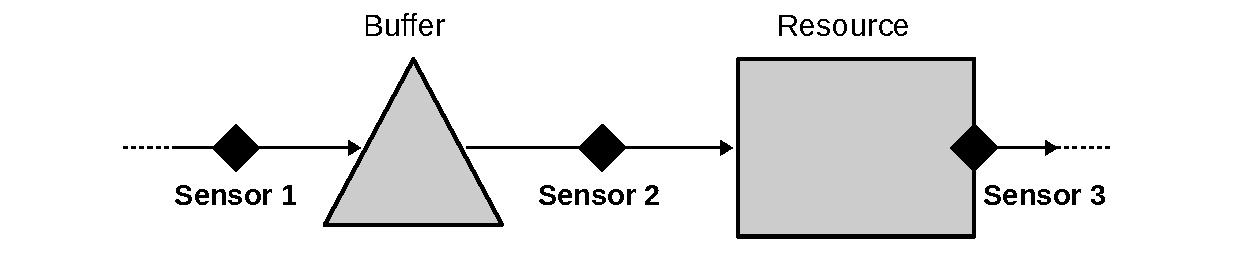
\includegraphics[width=1\textwidth]{Production_line_sensor_conf_thesis}
\caption[Three sensors configuration scheme]{Three sensors configuration scheme}
\label{fig:Three sensors configuration scheme}
\end{figure}
All the sensors are identical, and they all collect the same data, that are the job identification code (Case ID) and its passage instant (Timestamp). These are not the only fields composing the output event log, other attributes are associated, but they are not job-related fields, which have to be actively recorded by the sensors (like Case ID and timestamp), instead they keep track of the event and the sensor position. \\
%At the end of the thesis the topic of which indicators are obtainable if only two sensors are present in each stage is discussed. This situation could occur because of the breakage of one sensor or in the case of a placement design that aims to reduce time and costs related to implementation. 
\section{Considered process variations}
\subsection{Variation classifications}
The issue of process variation has been addressed in Process Mining, in particular within the wider topic of Streaming Process Discovery (see section \ref{Auto-update of process models using Process Mining}), that is the construction of models based not on finite event logs but on streams of events. Indeed, in the long term, an event stream relative to a process monitored in real time could be susceptible to concept drifts, which are “\textit{situations where the process is changing while being analyzed}” \cite{Aalst16}. \\
In \cite{BoseR.P.J.C.2011Hcdi} by Bose et al., concept drifts are classified based on three criteria. 
\subparagraph{Classification on perspective} It focuses on where the change occurs, indicating not the physical location but the level of variation. Three categories are identified:
\begin{itemize}
\item \textbf{Control-flow perspective}: this class includes structural changes, such as insertions, deletions, substitutions, and reordering of process components. For example, inserting new stages in the line, or adding new product types, cause variations of the model structure itself. 
\item \textbf{Data perspective}: this class includes changes related to requirements, usages, a data generation. For example, the enabling the execution of a task without the information request previously needed. 
\item \textbf{Resource perspective}: this class includes changes in roles and behaviors of resources. These variations influence the executions of a process, for example a resource capacity increase in the bottleneck can make the throughput increase if the process is unstable (i.e. production-constrained), or, in a multi-resource stage, a machine disabling makes the stage slower and raises its utilization.
\end{itemize}
\subparagraph{Classification on duration} As the name suggests, classification on duration aims to classify the variations based on their durations. Two categories are identified:
\begin{itemize}
\item \textbf{Momentary changes}: variation lifespans are short and may affect few activities, being not enough durable to influence the whole process. (Figure \ref{fig:Momentary change})
\item \textbf{Permanent changes}: variations lifespans are long-lasting, to the point that can be considered permanent. These changes usually affect all the process activities. (Figure \ref{fig:Permanent change})
\end{itemize}
\begin{figure}[H]
  \centering
  \begin{subfigure}[b]{0.4\textwidth}
    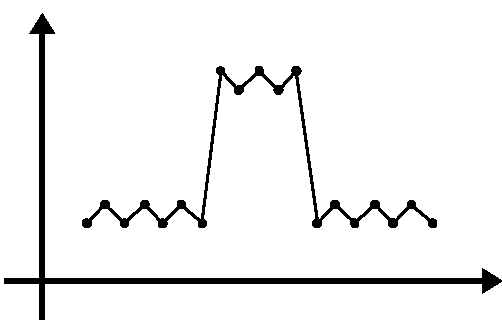
\includegraphics[width=\textwidth]{Momentary_change}
    \caption{Momentary change}
    \label{fig:Momentary change}   
  \end{subfigure}
  \hspace{0.1\textwidth}
  \begin{subfigure}[b]{0.4\textwidth}
    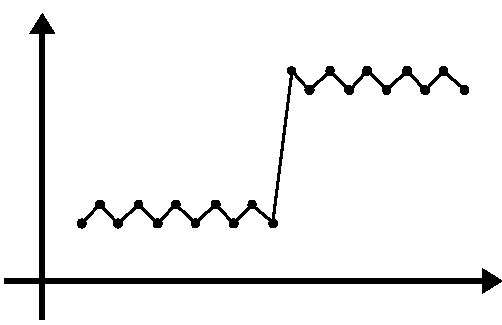
\includegraphics[width=\textwidth]{Permanent_change}
    \caption{Permanent change}
    \label{fig:Permanent change}
  \end{subfigure}             
  \caption{Change classification on duration}
  \label{fig:Change classification on duration}
\end{figure}
\subparagraph{Classification on nature} It focuses on the variation speed and frequency. Four categories are identified:
\begin{itemize}
\item \textbf{Sudden drift}: it includes variations consisting of instantaneous substitution of an existing process with a new one. This kind of change typically occurs in emergency circumstances, such as machine failures. (Figure \ref{fig:Sudden drift})
\item \textbf{Gradual drift}: it includes variations that occur without substituting the previous conditions, in other words it considers situations where different processes coexist for a certain time. This kind of variation is typical of planned organizational changes, such as the implementation of new procedures, without suddenly discontinuing the old ones. (Figure \ref{fig:Gradual drift})
\item \textbf{Incremental drift}: it includes variations that occur through small and incremental steps. This is typical of processes with slow machine deterioration over time. (Figure \ref{fig:Incremental drift})
\item \textbf{Recurring drift}: it includes variations which occur periodically, often with fixed frequency, followed by reinstatements of previous conditions. It is typical of processes characterized by seasonality. (Figure \ref{fig:Recurring drift})
\end{itemize}
\begin{figure}[H]
  \centering
  \begin{subfigure}[b]{0.4\textwidth}
    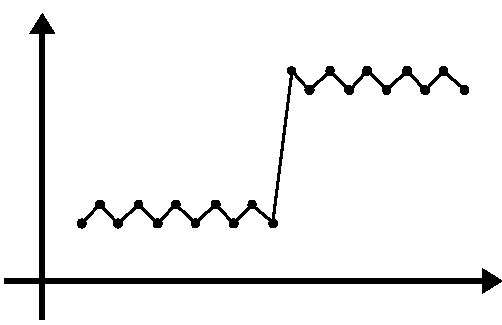
\includegraphics[width=\textwidth]{Sudden_change}
    \caption{Sudden drift}
    \label{fig:Sudden drift}   
  \end{subfigure}
  \hspace{0.1\textwidth}
  \begin{subfigure}[b]{0.4\textwidth}
    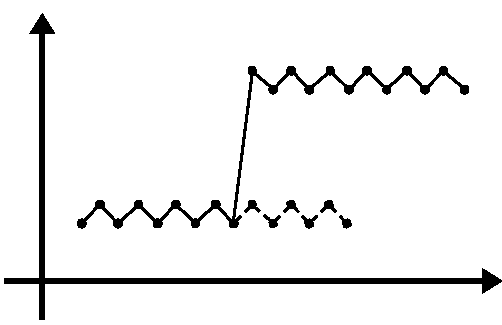
\includegraphics[width=\textwidth]{Gradual_change}
    \caption{Gradual drift}
    \label{fig:Gradual drift}
  \end{subfigure}
  \begin{subfigure}[b]{0.4\textwidth}
    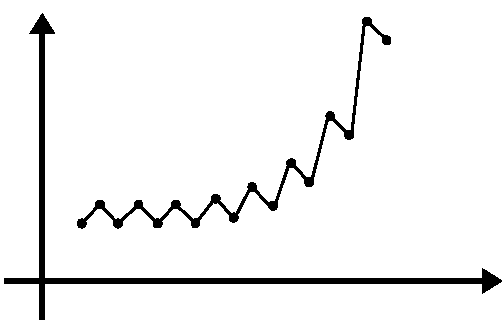
\includegraphics[width=\textwidth]{Incremental_change}
    \caption{Incremental drift}
    \label{fig:Incremental drift}
  \end{subfigure}
  \hspace{0.1\textwidth}
  \begin{subfigure}[b]{0.4\textwidth}
    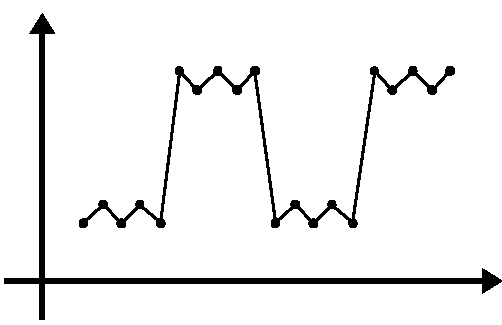
\includegraphics[width=\textwidth]{Recurring_change}
    \caption{Recurring drift}
    \label{fig:Recurring drift}
  \end{subfigure}
  \caption{Change classification on nature}
  \label{fig:Change classification on nature}
\end{figure}
\subsection{Considered variations}
In this thesis two variation types are considered:
\begin{itemize}
\item \textbf{Processing time variation in a resource}: a machine in a stage is subject to a sudden production capacity growth or loss, causing, respectively, a decrease or an increase of time needed to process a job in the stage. A capacity growth in a stage may occur in case of a machine substitution with a new and more efficient one. On the other side, a capacity loss may occur when an unnoticed resource deterioration is not adequately addressed by maintenance and abruptly affects the machine, slowing its production.
\item \textbf{Buffer capacity variation}: a buffer in a stage is subject to a sudden capacity limit growth or loss. This kind of variation may occur in a plug-and-play context, where buffers can expand or shrink based on the stage requirements, aiming to minimize blocking and starvation along the line. 
\end{itemize}
Therefore, according to the previous categorization, the variations considered in this dissertation are limited to stage-related, permanent, sudden changes. It is to be noted that the expression “stage-related” is used as the adaptation to a manufacturing context of the resource-perspective category, part of the classification on perspective. Indeed, in manufacturing the term resource is often used as synonym of machine, yet a resource-change, as meant above, can occur to any stage component, including buffers: a buffer capacity variation does not affect the model structure or the data requirement and usage, but influences stage behaviors and, so, the process execution, which is the distinctive trait of a resource-perspective variation. 